\documentclass[10pt,letterpaper]{article}
\usepackage{amsmath,amssymb}
\usepackage{color}
\usepackage{graphicx}
\usepackage{hyperref}
%\usepackage{url}
\usepackage{fullpage}
\usepackage[top=2cm, bottom=4.5cm, left=2.5cm, right=2.5cm]{geometry}
\renewcommand{\baselinestretch}{1.3}
%
% NOTE regarding macros %%
%
% Any macros defined for your paper should be contained in
% the top matter. Likewise, any environment definitions such
% as \newtheorem or \newenvironment should also go in the
% top matter.
%
% Do not \input your macros as separate files within your
% final version because more files make it harder for the
% editors and users to keep track of and/or modify and
% append your paper.
%
% Top matter is above and the beginning of the document below.
%
\begin{document}

\newpage


\title{Pandemic Modeling  -- Ebola, COVID-19, and Many More- a final project assignment written by Dr. J. Wang and adapted for Math 1550 at Wentworth}
\date{Posted on November 14, 2020}




\markboth{Pandemic Modeling}{Pandemic Modeling}


%\makeStitlePDFLaTex

\maketitle

\section*{DIRECTIONS and DELIVERABLES}

\begin{itemize}



\item There are three deliverables for your final project which you can do by yourself or with one other person:
\begin{itemize}
\item A final paper which is answering the three questions at the end of this reading. This is worth 10\% of your grade per the syllabus and is due on or by Study Day, Wed. Dec. 9 by 11:59 pm. The paper needs to be written in .tex so please submit a zip folder with your .tex file, the pdf that the .tex file generates and other files (images, python, etc).

\item A url to a video where you answer question 3. This is worth 5\% of your grade per the syllabus and is due on or by the last day of class  Dec. 8 by 11:59 pm. Your recording should be between 8 and 10 minutes. (So if you are doing this with one other person then your total time is still 8-10 minutes.)
You can use zoom to record for example if you are doing this with a partner.

\item Your slides written in LaTeX of your video presentation. (Submit a zip folder with your .tex file, the pdf that the .tex file generates and other files (images, python, etc). This is worth 5\% of your grade per the syllabus and is due on or by the last day of class  Dec. 8 by 11:59 pm. 

\end{itemize}
\item You need to let me know on or by Friday, Nov. 20 if you are doing the final paper, slides and video presentation by yourself or with 1 other person.
 I would prefer you do it  with a partner but it is okay if you want to do it by yourself. 
 
 \item Your grade on the paper, slides and video will be divided (approximately) into thirds based on the following rubric:
(i) Quality of presentation (points awarded for creativity, innovation, and artistic air)
(ii) Quality of the mathematics and research conducted
(iii) Quality of the paper (well-written, organized, readable, in your own words, appropriately referenced, etc.)



\end{itemize}

\section*{STATEMENT}
On December 31, 2019, the city of Wuhan in China reported an outbreak of a novel coronavirus (COVID-19). It is the seventh member of the coronavirus family, together with MERS-CoV and SARS-CoV, that can spread to humans \cite{CDC2020}. The virus is spreading rapidly. As of April 20, 2020, over 2.4 million people worldwide have been infected, spanning 210 countries and territories. The World Health Organization (WHO) has declared the outbreak as a pandemic. 

The word `pandemic' comes from the Greek word `pandemos', meaning ``pertaining to all people''. The Greek word `pan' means ``all'' and `demos' means ``people''. Pandemics are usually caused by an infectious agent that is capable of rapidly spreading. An epidemic is specific to one city, region, or country, but a pandemic spreads beyond national borders, possibly worldwide. The 1918 Spanish flu was the worst pandemic in modern human history. It infected 500 million people around the world and resulted in the deaths of over 50 million people \cite{CDC2019}. Increased travel and mobility have increased the likelihood of new diseases spreading. Figure~\ref{fig:pandemics} lists the major epidemics and pandemics that have occurred over time. The recent ones are SARS, swine flu, Ebola, MERS, and COVID-19.

Infectious disease modeling is an essential part of the effort to minimize the spread. A well-designed model not only can help predict the likely course of an epidemic, but also can reveal the most promising and realistic strategies for containing it.

{\bf How can we use mathematical models and differential equations to study the spread of coronavirus?}

\begin{figure}[!htb]
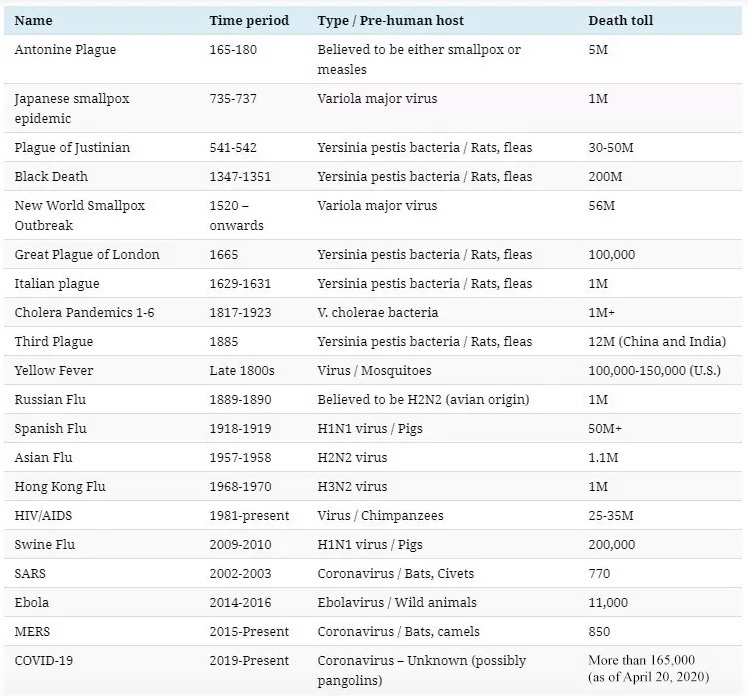
\includegraphics[width=6in]{pandemics2.jpg}
\centering
\caption{\label{fig:pandemics}Major epidemics and pandemics in human history, modified from \cite{Pandemic2020}.}
\end{figure}

\section*{Mathematical modeling -- the SIR model}
Let's first examine differential equation models in epidemiology. Epidemiology is the study of the distribution and causes of disease in populations. The spread of infectious diseases, such as measles and malaria, can be modeled by a system of nonlinear differential equations. The simplest model is the {\bf SIR} model (Susceptible-Infected-Recovered). The model makes several basic assumptions:
\begin{enumerate}
\item[A1.] The total population is constant.
\item[A2.] Once an individual has been infected and subsequently recovered, that individual cannot be re-infected, such as in the case of measles, mumps, and smallpox.
\item[A3.] The rate of transmission of the disease is proportional to the number of encounters between susceptible and infected individuals.
\item[A4.] The rate at which infected individuals recover is proportional to the number of infected.
\end{enumerate}

As the first step in the modeling process, we identify the independent and dependent variables. The independent variable is time $t$, measured in days. The dependent variables are the numbers of individuals in each group, each as a function of time.

\begin{align*}
s(t) &= \textnormal{the number of susceptible individuals} \\ 
i(t) &= \textnormal{the number of infected individuals} \\ 
r(t) &= \textnormal{the number of recovered individuals} \\ 
s(t)&+i(t)+r(t) = N \textnormal{ (the total population)}
\end{align*}

It may seem more natural to work with population counts, but some of our calculations will be simpler if we use the fractions instead. Therefore, we normalize the dependent variables by the total population to represent the fraction of the total population in each group. The two sets of dependent variables are proportional to each other, so either set will give us the same information about the progress of the epidemic.

\begin{align*}
S(t) &= s(t)/N = \textnormal{the fraction of susceptible individuals} \\
I(t) &= i(t)/N = \textnormal{the fraction of infected individuals} \\
R(t) &= r(t)/N = \textnormal{the fraction of recovered individuals}\\
S(t)&+I(t)+R(t) = 1
\end{align*}


The SIR model is illustrated schematically in Figure~\ref{fig:SIR}, and described by the nonlinear system of ODEs below, where $a$ is the transmission rate and $r$ is the recovery rate. 
\begin{align}
S'(t) &= -a S I \\
I'(t) &= a S I - r I \\
R'(t) &= r I
\end{align}

\begin{figure}[htb]
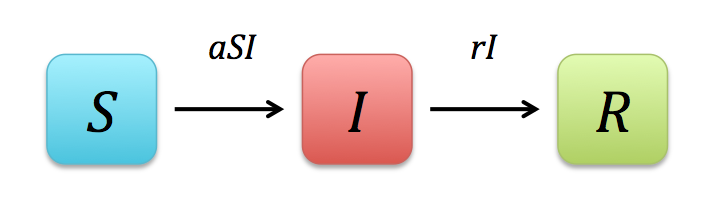
\includegraphics[width=3.5in]{SIR}
\centering
\caption{\label{fig:SIR}The SIR model.}
\end{figure}

To understand this model, let's analyze the differential equations and parameters. The {\bf transmission rate} $a$ is the product of two factors:  the rate of contact and probability of transmission. $a$ describes the fraction of those contacts that may result in infection, or it can be interpreted as the expected number of people an infected person infects per day. The function $\lambda(I)=aI$ is the rate at which susceptible individuals become infectious, called the {\bf force of infection}. The rate of change of the susceptible population is negative the force of infection times the number of susceptible, leading to (1).

The {\bf recovery rate} $r$ is the rate at which infected individuals get over the disease, that is the proportion of infected recovering per day, thus the rate of change of the recovered population is $rI$, leading to (3). Importantly, the parameter $r$ is measured in time$^{-1}$ and $1/r$ can be interpreted as the {\bf average time to recover}, or the number of days an infected person has and can spread the disease.

Can you explain (2)?\\

In the GeoGebra App \cite{GeoGebra1}, let's solve the nonlinear system (using `NSolveODE'), plot the solutions, and visualize the interaction of the three groups. The GeoGebra tutorials are available online \cite{GeoGebra2}. Consider the initial population fractions $S(0)=0.99, I(0)=0.01, R(0)=0 \; (S+I+R=1)$, $a=1, r=0.2$, and a time period of 30 days. An example demonstration is provided in \cite{Wang2020} with a screenshot in Figure~\ref{fig:GeoGebra}. Adjust the parameters values to examine different behaviors and view the changes in action. What do you observe by increasing or decreasing $a$? 

\begin{figure}[htb]
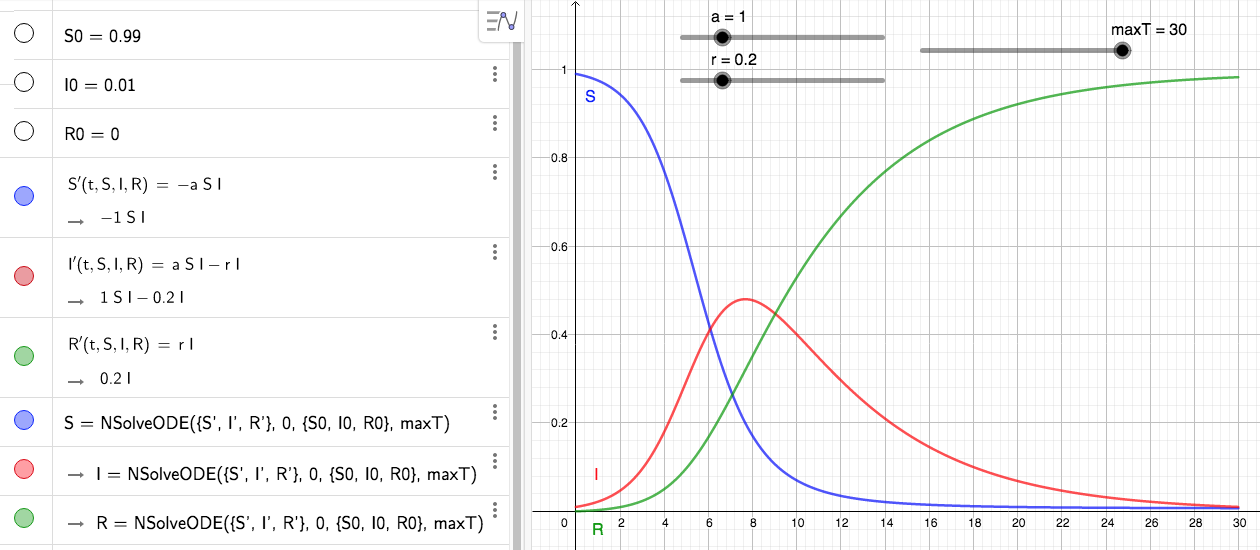
\includegraphics[width=5.4in]{GeoGebra}
\centering
\caption{\label{fig:GeoGebra}A screenshot of GeoGebra dynamic constructions.}
\end{figure}

\section*{Basic Reproduction Number $R_0$}
The {\it  basic reproduction number\/} $R_0$, ``$R$ naught'', is introduced to measure the transmission potential of a disease. It is the expected number of secondary infections produced by a single infective. For example, if the $R_0$ for measles in a population is 16, then we would expect each new case of measles to produce 16 new secondary cases over the period of time during which the infected individual can actually spread the disease. $R_0$ is affected by several factors: the rate of contacts in the host population, the probability of infection being transmitted during contact, and the duration of infectiousness. In the SIR model described above, 
\begin{equation}
R_0=\frac{a}{r}.
\end{equation}

$R_0$ is essentially a metric of how contagious a disease is. It can capture three basic scenarios, illustrated in Figure~\ref{fig:R0}.
\begin{figure}[htb]
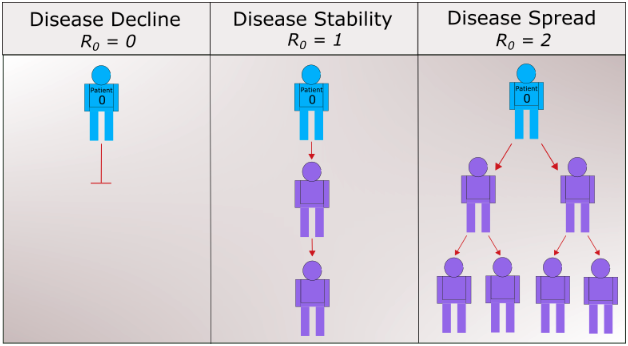
\includegraphics[width=3.7in]{R0}
\centering
\caption{\label{fig:R0}Basic reproduction number $R_0$ \cite{COVID2020}.}
\end{figure}

If $R_0 < 1$, on average, an infected person infects less than one person. The disease is expected to stop spreading. If $R_0 = 1$, an infected person infects an average of one person.
The disease spread is stable, or endemic. If $R_0 > 1$, on average, an infected person infects more than one person. The disease is expected to increasingly spread in the absence of intervention. Here is the estimated $R_0$ for several diseases \cite{Pandemic2020}. Measles tops the list, being the most contagious with a $R_0$ range of 12-18. Early estimates of $R_0$ for COVID-19 vary in the range of 2-3. \bigskip

\section*{Answer the following questions for your final project}

\begin{enumerate}
\item Examine (1) and (2) again
\begin{equation*} 
\frac{dS}{dt} = -a S I, \quad \frac{dI}{dt} = a S I - r I 
\end{equation*}

\begin{enumerate}
\item According to the differential equation for $dI/dt$, under what conditions will $I(t)$ be increasing? decreasing? What does this mean about the spread of the disease? Using this result, explain whether quarantine will be effective against the disease.

\item Use the chain rule to show that 
\begin{equation}
\frac{dI}{dS}=-1+\frac{1}{R_0S}
\end{equation}

Two features of this new equation are particularly worth noting: 
\begin{itemize}
\item The only parameter that appears is $R_0$, the reproduction number.
\item The equation is independent of time. That is, what we learn about the relationship between $S$ and $I$ must be true for the entire duration of the epidemic.
\end{itemize}
Compute $d^2I/dS^2$. Determine when the number of infected will begin to decrease. \\
Compare this to your reslult from (a).

\item Show that $I$ must have the form 
\begin{equation}
I=-S+\frac{1}{R_0}\ln{S} + C
\end{equation}
by using separation of variables (we separation of variabes a while ago and only once in class) where $C$ is a constant.

\item For a disease such as COVID-19, $I(0)$ is approximately 0 and $S(0)$ is approximately 1. A long time after the onset of the epidemic, we have $I(\infty)$ approximately 0 again, and $S(\infty)$ has settled to its steady state value, observable as the fraction of the population that did not get the disease. Explain why $$R_0=\frac{\ln{S_\infty}}{S_\infty-1}.$$

\item Describe the meaning and significance of ``herd immunity''. How can vaccination lead to herd immunity?

\end{enumerate}

\item Recovered individuals may lose their immunity and become re-infected, such as in the case of malaria and tuberculosis, as well as COVID-19. We add a new assumption.
\vspace*{.2 true cm}

A5. Re-infection occurs at a rate proportional to the population of recovered individuals. Call this proportional parameter $b$. 

\vspace*{.2 true cm}
Sketch a schematic diagram similar to Figure~\ref{fig:SIR}. Modify (1)-(3) and set up the new model -- the {\bf SIRS} model, with parameters $a$, $r$, and $b$.

\item In reality, deaths may occur due to the disease. For simplicity, let's only consider deaths from the infected group $I$, with a death rate $c$. 
\begin{enumerate}
\item Modify your previous diagram and model in 2, including four differential equations with the fourth being $D'(t)=\ldots$, and parameters $a$, $r$, $b$, and $c$. 
\item Pick one pandemic from the list in Figure~\ref{fig:pandemics} and a region, such as a city or a country. Research into the data available and obtain reasonable estimates of the parameters $a$, $r$, $b$, and $c$, as well as initial conditions $S(0)$ and $I(0)$. \textbf{Include your data and cite your source(s).} Set $R(0)=D(0)=0$. Note that $S+I+R+D=1$.
\item Solve your model with these parameter values and visualize the solutions in GeoGebra (\textbf{Or do this using Python).} If you use Geogebra, Include a sharable link to your work.  If you use Python include your code( .py file) and figure(s). Describe the behavior of the solutions. Compare your results with the real data. Does your model seem reasonable? Explain. 
\end{enumerate}

\end{enumerate}

\bigskip
Other models include SEIR, SEIS, SEAIR, MSIR, MSEIR, and MSEIRS. For many infections, there is an incubation period during which individuals have been infected but are not yet infectious themselves. During this period the individual is in class E (for exposed), leading to the SEIR model. The SEIS model is like the SEIR except that no immunity is acquired at the end. In the E class, a significant number of persons may never develop symptoms, but they are capable of transmitting the disease, introducing an additional compartment A, and thus SEAIR. For many infections, such as measles, babies are not born into the susceptible compartment but are immune to the disease for the first few months of life due to protection from maternal antibodies. The M class contains infants with maternally derived immunity (or passive immunity). The MSEIRS model is similar to the MSEIR, but the immunity in the R class would be temporary, so that individuals would regain their susceptibility when the temporary immunity ended. 

\begin{thebibliography}{98}

\bibitem{CDC2020} Centers for Disease Control and Prevention. 2020. Human Coronavirus Types. \href{https://www.cdc.gov/coronavirus/types.html}{https://www.cdc.gov/coronavirus/types.html}. Accessed 10 May 2020.

\bibitem{CDC2019} Centers for Disease Control and Prevention. 2019. 1918 influenza pandemic (H1N1 virus). 
\href{https://www.cdc.gov/flu/pandemic-resources/1918-pandemic-h1n1.html}{https://www.cdc.gov/flu/pandemic-resources/1918-pandemic-h1n1.html}. Accessed 10 May 2020.

\bibitem{Pandemic2020} A visual history of pandemics. 2020. 
\href{https://www.weforum.org/agenda/2020/03/a-visual-history-of-pandemics}{https://www.weforum.org/agenda/2020/03/a-visual-history-of-pandemics}. Accessed 10 May 2020.

\bibitem{GeoGebra1} GeoGebra Math Apps. \href{https://www.geogebra.org}{https://www.geogebra.org}. Accessed 10 May 2020.

\bibitem{GeoGebra2} GeoGebra Tutorials. \href{https://www.geogebra.org/m/XUv5mXTm}{https://www.geogebra.org/m/XUv5mXTm}. Accessed 10 May 2020.

\bibitem{Wang2020} Wang, J. 2020. GeoGebra example: \href{https://www.geogebra.org/classic/zumeuffq}{https://www.geogebra.org/classic/zumeuffq}. Accessed 10 May 2020.

\bibitem{COVID2020} How COVID-19 and other infectious diseases spread: mathematical modeling. 2020. 
\href{https://triplebyte.com/blog/modeling-infectious-diseases}{https://triplebyte.com/blog/modeling-infectious-diseases}. Accessed 10 May 2020.

\end{thebibliography}


\end{document}
